\begin{enumerate}[label=\thesubsection.\arabic*.,ref=\thesubsection.\theenumi]
\numberwithin{equation}{enumi}

\item Consider a state-variable model of a system 
\begin{align}
\myvec{\dot{x_{1}}\\\dot{x_{2}}}
=
\myvec{0&1\\-\alpha&-2\beta}\myvec{x_{1}\\x_{2}}
+
\myvec{b_{1}\\b_{2}}  r
\end{align}
\begin{align}
y
=
\myvec{1&0}\myvec{x_{1}\\x_{2}}
\end{align}
where y is the output, and r is the input.
%
Find the the system transfer function $H(s)$.

\solution The state space model is given by
\begin{align}
\dot{X} = AX + BU
\end{align}
\begin{align}
Y = CX + DU
\end{align}
%
The transfer function for the state space model is:
\begin{align}
H(s) = C(sI - A)^{-1}B + D
\end{align}
\begin{align}
\implies H(s) = \frac
{
\myvec{1&0}\myvec{s+2\beta&1\\-\alpha&s}\myvec{b_{1}\\b_{2}}
}
{
s(s+2\beta) + \alpha
}
\end{align}
\begin{align}
= \LARGE{\frac{b_{1}(s+2\beta) + b_{2}}{s^{2}+2s\beta+\alpha}}
\end{align}
\begin{align}
   \implies H(s) = \LARGE{\frac{b_{1}s}{s^{2}+2s\beta+\alpha}} + \LARGE{\frac{2b_{1}\beta + b_{2}}{s^{2}+2s\beta+\alpha}}
\end{align}
%\begin{table}[!ht]
%\centering
%\begin{enumerate}[label=\thesubsection.\arabic*.,ref=\thesubsection.\theenumi]
\numberwithin{equation}{enumi}

\item Consider a state-variable model of a system 
\begin{align}
\label{eq:ee18btech11011_state}
\myvec{\dot{x_{1}}\\\dot{x_{2}}}
=
\myvec{0&1\\-\alpha&-2\beta}\myvec{x_{1}\\x_{2}}
+
\myvec{b_{1}\\b_{2}}  r
\end{align}
\begin{align}
y
=
\myvec{1&0}\myvec{x_{1}\\x_{2}}
\end{align}
where y is the output, and r is the input.
%
\item List the various state matrices in \eqref{eq:ee18btech11011_state}

\item Find the the system transfer function $H(s)$.

\solution From \eqref{eq:ee18btech11004_state} and ,
%
\eqref{eq:ee18btech11004_siso}, 
the transfer function for the state space model is
\begin{align}
H(s) &= C(sI - A)^{-1}B + D
\\
& = \frac
{
\myvec{1&0}\myvec{s+2\beta&1\\-\alpha&s}\myvec{b_{1}\\b_{2}}
}
{
s(s+2\beta) + \alpha
}
\\
&= {\frac{b_{1}(s+2\beta) + b_{2}}{s^{2}+2s\beta+\alpha}}
\\
   \implies H(s) &= {\frac{b_{1}s}{s^{2}+2s\beta+\alpha}} + \LARGE{\frac{2b_{1}\beta + b_{2}}{s^{2}+2s\beta+\alpha}}
\label{eq:ee18btech11011_second}
\end{align}
%\begin{table}[!ht]
%\centering
%\begin{enumerate}[label=\thesubsection.\arabic*.,ref=\thesubsection.\theenumi]
\numberwithin{equation}{enumi}

\item Consider a state-variable model of a system 
\begin{align}
\label{eq:ee18btech11011_state}
\myvec{\dot{x_{1}}\\\dot{x_{2}}}
=
\myvec{0&1\\-\alpha&-2\beta}\myvec{x_{1}\\x_{2}}
+
\myvec{b_{1}\\b_{2}}  r
\end{align}
\begin{align}
y
=
\myvec{1&0}\myvec{x_{1}\\x_{2}}
\end{align}
where y is the output, and r is the input.
%
\item List the various state matrices in \eqref{eq:ee18btech11011_state}

\item Find the the system transfer function $H(s)$.

\solution From \eqref{eq:ee18btech11004_state} and ,
%
\eqref{eq:ee18btech11004_siso}, 
the transfer function for the state space model is
\begin{align}
H(s) &= C(sI - A)^{-1}B + D
\\
& = \frac
{
\myvec{1&0}\myvec{s+2\beta&1\\-\alpha&s}\myvec{b_{1}\\b_{2}}
}
{
s(s+2\beta) + \alpha
}
\\
&= {\frac{b_{1}(s+2\beta) + b_{2}}{s^{2}+2s\beta+\alpha}}
\\
   \implies H(s) &= {\frac{b_{1}s}{s^{2}+2s\beta+\alpha}} + \LARGE{\frac{2b_{1}\beta + b_{2}}{s^{2}+2s\beta+\alpha}}
\label{eq:ee18btech11011_second}
\end{align}
%\begin{table}[!ht]
%\centering
%\begin{enumerate}[label=\thesubsection.\arabic*.,ref=\thesubsection.\theenumi]
\numberwithin{equation}{enumi}

\item Consider a state-variable model of a system 
\begin{align}
\label{eq:ee18btech11011_state}
\myvec{\dot{x_{1}}\\\dot{x_{2}}}
=
\myvec{0&1\\-\alpha&-2\beta}\myvec{x_{1}\\x_{2}}
+
\myvec{b_{1}\\b_{2}}  r
\end{align}
\begin{align}
y
=
\myvec{1&0}\myvec{x_{1}\\x_{2}}
\end{align}
where y is the output, and r is the input.
%
\item List the various state matrices in \eqref{eq:ee18btech11011_state}

\item Find the the system transfer function $H(s)$.

\solution From \eqref{eq:ee18btech11004_state} and ,
%
\eqref{eq:ee18btech11004_siso}, 
the transfer function for the state space model is
\begin{align}
H(s) &= C(sI - A)^{-1}B + D
\\
& = \frac
{
\myvec{1&0}\myvec{s+2\beta&1\\-\alpha&s}\myvec{b_{1}\\b_{2}}
}
{
s(s+2\beta) + \alpha
}
\\
&= {\frac{b_{1}(s+2\beta) + b_{2}}{s^{2}+2s\beta+\alpha}}
\\
   \implies H(s) &= {\frac{b_{1}s}{s^{2}+2s\beta+\alpha}} + \LARGE{\frac{2b_{1}\beta + b_{2}}{s^{2}+2s\beta+\alpha}}
\label{eq:ee18btech11011_second}
\end{align}
%\begin{table}[!ht]
%\centering
%\input{./tables/ee18btech11011}
%\caption{}
%\label{table:ee18btech11011}
%\end{table}
\item Find the Damping ratio $\zeta$ and the Undamped natural frequency $\omega_{n}$ of the system.
\\
\solution Generally for a second order system the transfer function is given by \ref{eq:ee18btech11012_second}
%
\begin{align}
H(s) = \LARGE{\frac{\omega_{n}^2}{s^{2}+2s\zeta\omega_{n}+\omega_{n}^2}}
\end{align}
%
Comparing the denominator of the above with \eqref{eq:ee18btech11011_second},
%
\begin{align}
2\zeta\omega_{n} &= 2\beta,
\\
\omega_{n}^2 &= \alpha
\\
\implies \zeta &= \frac{\beta}{\sqrt{\alpha}} , \omega_{n} = \sqrt{\alpha}
\end{align}
%
\item Using Table \ref{table:ee18btech11012}, explain how the damping conditions depend upon $\alpha$ and  $\beta$.

%\item How do $\alpha$ and $\beta$ affect the system performance?  Explain through plots.
%\\
%\solution The following code plots Fig. \ref{fig:ee18btech11011}
%%
%\begin{figure}[!ht]
%	\begin{center}
%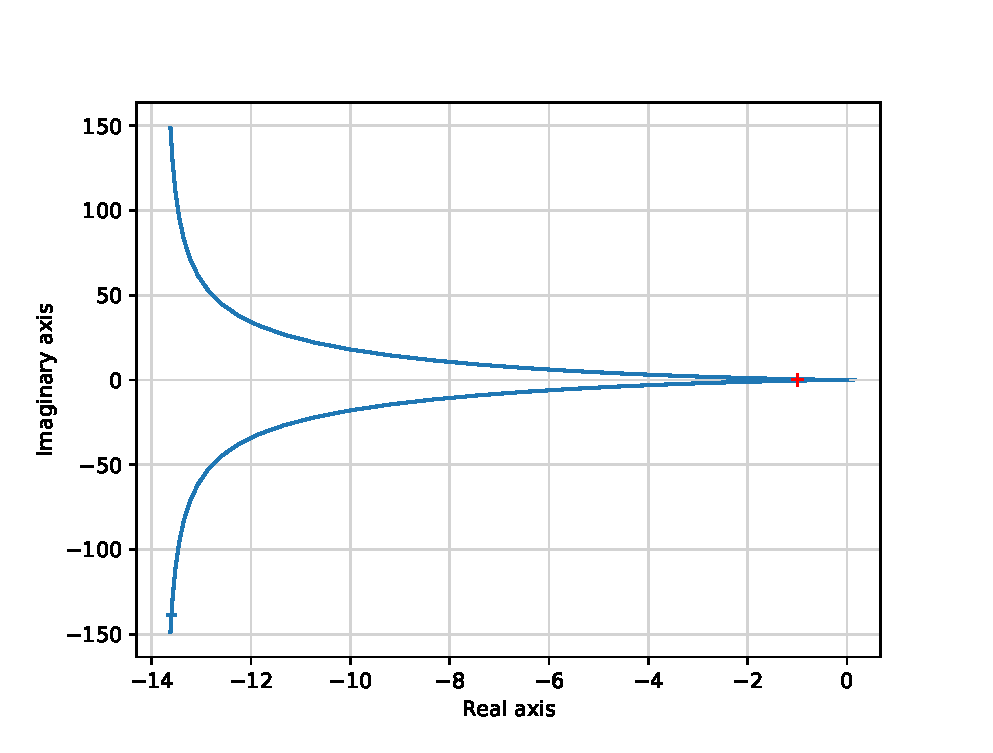
\includegraphics[width=\columnwidth]{./figs/ee18btech11011.eps}		
%	\end{center}
%\caption{}
%\label{fig:ee18btech11011}
%\end{figure}

\end{enumerate}


%\caption{}
%\label{table:ee18btech11011}
%\end{table}
\item Find the Damping ratio $\zeta$ and the Undamped natural frequency $\omega_{n}$ of the system.
\\
\solution Generally for a second order system the transfer function is given by \ref{eq:ee18btech11012_second}
%
\begin{align}
H(s) = \LARGE{\frac{\omega_{n}^2}{s^{2}+2s\zeta\omega_{n}+\omega_{n}^2}}
\end{align}
%
Comparing the denominator of the above with \eqref{eq:ee18btech11011_second},
%
\begin{align}
2\zeta\omega_{n} &= 2\beta,
\\
\omega_{n}^2 &= \alpha
\\
\implies \zeta &= \frac{\beta}{\sqrt{\alpha}} , \omega_{n} = \sqrt{\alpha}
\end{align}
%
\item Using Table \ref{table:ee18btech11012}, explain how the damping conditions depend upon $\alpha$ and  $\beta$.

%\item How do $\alpha$ and $\beta$ affect the system performance?  Explain through plots.
%\\
%\solution The following code plots Fig. \ref{fig:ee18btech11011}
%%
%\begin{figure}[!ht]
%	\begin{center}
%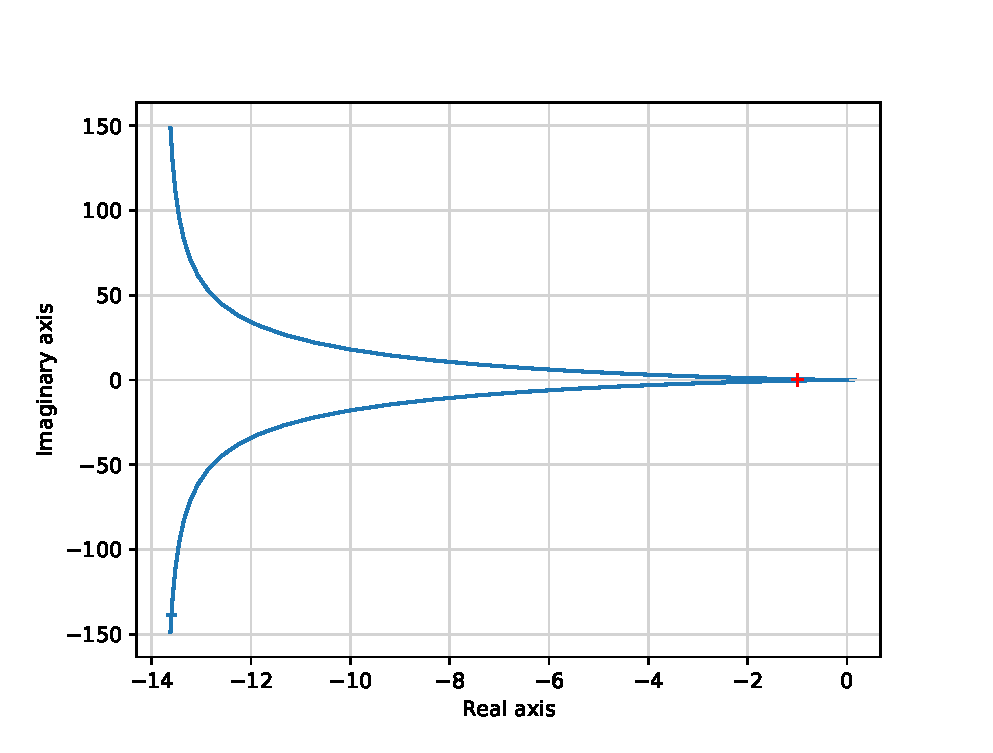
\includegraphics[width=\columnwidth]{./figs/ee18btech11011.eps}		
%	\end{center}
%\caption{}
%\label{fig:ee18btech11011}
%\end{figure}

\end{enumerate}


%\caption{}
%\label{table:ee18btech11011}
%\end{table}
\item Find the Damping ratio $\zeta$ and the Undamped natural frequency $\omega_{n}$ of the system.
\\
\solution Generally for a second order system the transfer function is given by \ref{eq:ee18btech11012_second}
%
\begin{align}
H(s) = \LARGE{\frac{\omega_{n}^2}{s^{2}+2s\zeta\omega_{n}+\omega_{n}^2}}
\end{align}
%
Comparing the denominator of the above with \eqref{eq:ee18btech11011_second},
%
\begin{align}
2\zeta\omega_{n} &= 2\beta,
\\
\omega_{n}^2 &= \alpha
\\
\implies \zeta &= \frac{\beta}{\sqrt{\alpha}} , \omega_{n} = \sqrt{\alpha}
\end{align}
%
\item Using Table \ref{table:ee18btech11012}, explain how the damping conditions depend upon $\alpha$ and  $\beta$.

%\item How do $\alpha$ and $\beta$ affect the system performance?  Explain through plots.
%\\
%\solution The following code plots Fig. \ref{fig:ee18btech11011}
%%
%\begin{figure}[!ht]
%	\begin{center}
%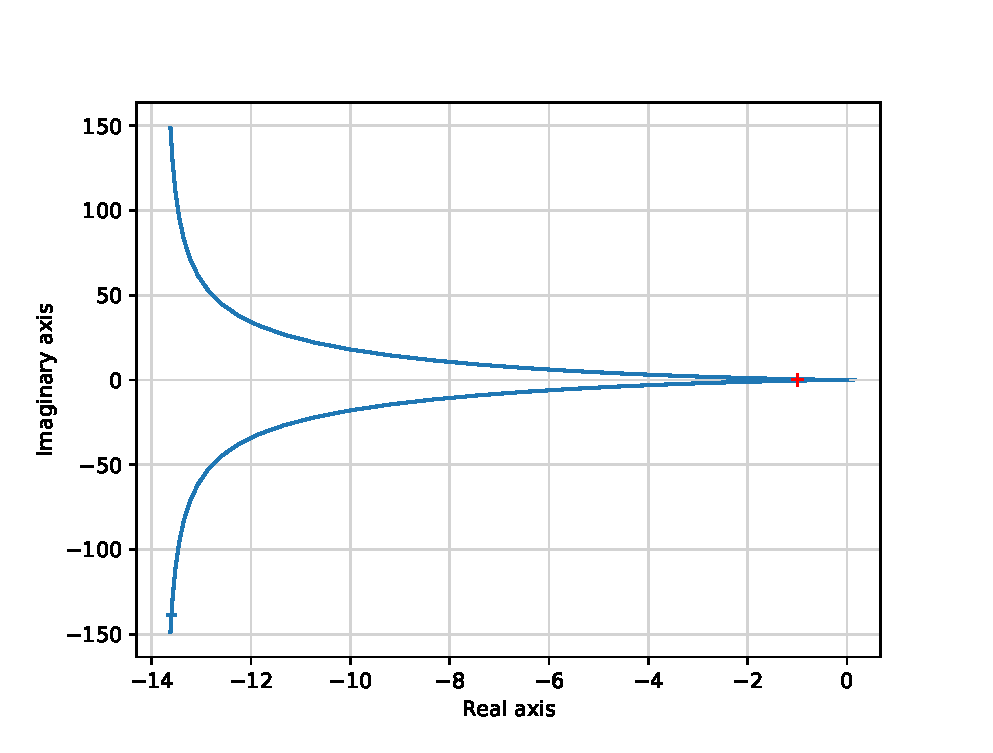
\includegraphics[width=\columnwidth]{./figs/ee18btech11011.eps}		
%	\end{center}
%\caption{}
%\label{fig:ee18btech11011}
%\end{figure}

\end{enumerate}


%\caption{}
%\label{table:ee18btech11011}
%\end{table}
\item Find the Damping ratio $\zeta$ and the Undamped natural frequency $\omega_{n}$ of the system.
\\
\solution
Generally for a second order system the transfer function is given by
\begin{align}
H(s) = \LARGE{\frac{\omega_{n}^2}{s^{2}+2s\zeta\omega_{n}+\omega_{n}^2}}
\end{align}
Now from the transfer function we got we can see that our system is bandpass and lowpass combination but the comaprison of denominator of our transfer function to the general transfer function is still valid.
\begin{align}
\therefore 2\zeta\omega_{n} = 2\beta,
\end{align}
\begin{align}
\omega_{n}^2 = \alpha
\end{align}
\begin{align}
\implies \zeta = \frac{\beta}{\sqrt{\alpha}} , \omega_{n} = \sqrt{\alpha}
\end{align}
\item What is the significance of $\zeta$ and  $\omega_{n}$? Explain through plots.
\item How do $\alpha$ and $\beta$ affect the system performance?  Explain through plots.
\\
\solution The following code plots Fig. \ref{fig:ee18btech11011}
%
\begin{figure}[!ht]
	\begin{center}
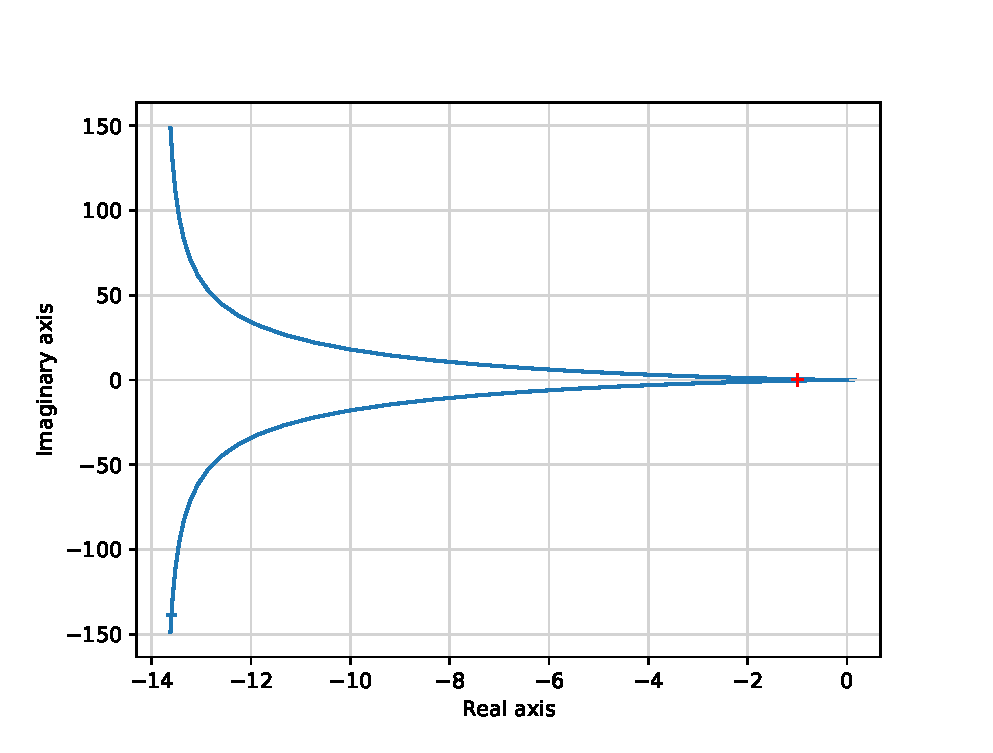
\includegraphics[width=\columnwidth]{./figs/ee18btech11011.eps}		
	\end{center}
\caption{}
\label{fig:ee18btech11011}
\end{figure}

\end{enumerate}

